\documentclass[12pt,a4paper]{amsart}
\usepackage{amsfonts}
\usepackage{amsthm}
\usepackage{amsmath}
\usepackage{amscd}
\usepackage[latin2]{inputenc}
\usepackage{t1enc}
\usepackage[mathscr]{eucal}
\usepackage{indentfirst}
\usepackage{graphicx}
\usepackage{graphics}
\usepackage{pict2e}
\usepackage{epic}
\numberwithin{equation}{section}
\usepackage[margin=2.9cm]{geometry}
\usepackage{epstopdf} 

 \def\numset#1{{\\mathbb #1}}

\usepackage{caption}
\usepackage{subcaption}
\usepackage{float} 

\theoremstyle{plain}
\newtheorem{Th}{Theorem}[section]
\newtheorem{Lemma}[Th]{Lemma}
\newtheorem{Cor}[Th]{Corollary}
\newtheorem{prop}[Th]{Proposition}

 \theoremstyle{definition}
\newtheorem{Def}[Th]{Definition}
\newtheorem{Conj}[Th]{Conjecture}
\newtheorem{Rem}[Th]{Remark}
\newtheorem{?}[Th]{Problem}
\newtheorem{Ex}[Th]{Example}

\newcommand{\im}{\operatorname{im}}
\newcommand{\Hom}{{\rm{Hom}}}
\newcommand{\diam}{{\rm{diam}}}
\newcommand{\ovl}{\overline}
%\newcommand{\M}{\mathbb{M}}

\begin{document}

\title{Sample paper}


\author[A. Nanyanzi]{Alice Nanyanzi}

\address{AIMS-South Africa \\ Department of Mathematics \\
Cambridge MA 02139 \&  E\"{o}tv\"{o}s Lor\'{a}nd University \\ Department of Computer 
Science \\ H-1117 Budapest
\\ P\'{a}zm\'{a}ny P\'{e}ter s\'{e}t\'{a}ny 1/C \\ Hungary} 

\email{alicenanyanzi@aims.ac.za}














 \subjclass[2010]{Primary: 05C??. Secondary: 05C??}



 \keywords{sample paper} 



\begin{abstract} The heat kernel of a graph is the fundamental solution to the heat diffusion equation associated with Laplacian of a graph.  The heat kernel can also be viewed as a description of flow of information (or heat in this case) over the edges of the graph with time. It is computed by exponentiating the Laplacian eigen-system with time. In this paper, we extend this concept by considering diffusion on the graph along direct edges as well as along indirect edges which we refer to as long-range interactions. The heat kernel resulting as a fundamental solution to the mentioned type of diffusion is what we refer to as the generalised heat kernel. We account for the long-range interactions in two ways namely; the Mellin and Laplace transforms of the Laplacian. We then perform experiments on the generalised heat kernel which is then followed by explanation of results.
\end{abstract}

\maketitle

\section{Introduction} Dynamics on networks such as diffusion, consensus, synchronisation, etc. have recently attracted attention of researchers. This is because of their applicability in various areas such as modelling of epidermic spread, diffusion of information in social networks, among others.

It has been observed in modelling of dynamic processes on networks that the substance in consideration say information, heat, disease, rumour, and many more do spread that the flow is not only along direct edges of the networks but also through indirect interactions. Estrada explored ways of accounting for the indirect or long-range interactions by use of the social distance analogy which was associated with constraints in selection of the conductance parameter $x$ \cite{estrada2011epidemic}. In his subsequent work, elegant approaches were put forward based on the Mellin and Laplace transforms of the graph Laplacian \cite{estrada2012path,estrada2017long}. 

Diffusion is, among others, the movement of substance from a region of high concentration to a region of low concentration. Such substance include heat, gas, etc. \cite{newman2010}.

Diffusion process over networks is one of the methods used in developing simple models that depict the spread of infections in a population, dissemination of information over social network for instance social network marketing, spread of heat over a conductor, among others. A number of models based on diffusion process have been developed and documented in \cite{estrada2011epidemic,kasprzak2012diffusion,lopez2008diffusion}.

The diffusion kernel which is the fundamental solution of the heat equation is quite an important aspect in the study of diffusion on networks. It has been used as a means of characterising of networks, in graph clustering, among others \cite{xiao2009graph}. The heat kernel in these cases is based on diffusion that occurs along the edges of a network. In this work, however, we explore the heat kernel for which diffusion occurs through both short-range (over the edges) and long-range interactions. We call this the generalised heat kernel.


\section{Heat Diffusion Model}
Let $G=(V,E)$ be a simple connected undirected graph with vertex set $V$ and edge set $E$. Suppose we randomly select a few nodes ( that is, sources) to which we assign specific amounts of heat as in vector $\phi_0$. With the heat diffusion coefficient, $\varepsilon \in [0,1]$ which controls the rate of diffusion. When $\varepsilon$ tends to $0$, heat transfer among nodes becomes difficult and as a result, heat does not spread to each of the nodes with in the network. However, as $\varepsilon$ tends to $1$, heat spreads rapidly among nodes and thus, with out loss, heat is distributed to all nodes in the network.

% At any time $t$, we obtain the quantities of heat,$\phi_t$, at each node, . The spread of heat is considered to occur following the edges connecting nodes, that is to say, through direct interactions.  
% The process of heat spread over the network can therefore be modelled by
% \begin{equation}
% \frac{d\phi_i}{dt} = \varepsilon \sum_j (\mathbf{A}_{ij} - \delta_{ij} k_i) \phi_j,
% \label{difusion}
% \end{equation}
% where $\mathbf{A}$ is the adjacency matrix whose elements $A(i,j)$ is $1$ for node $i$ adjacent to node $j$ and $0$ otherwise. $k_i$ is the degree of node $i$, and $\delta_{ij}$ is the Kronecker delta whose value is $1$ if $i=j$ and $0$ otherwise. 

Consider a simple undirected network. Suppose we have a quantity $\phi_i$ of a substance on a vertex $i$ at time $t$. Suppose the substance moves along edges from node $j$ to an adjacent node $i$ at a rate $\varepsilon(\phi_j -\phi_i)$, where $\varepsilon$ is the diffusion constant ($\varepsilon>0$). The amount of substance moving from $j$ to $i$ in a small time interval $dt$ is $C(\phi_j -\phi_i)~dt$. Then the rate at which substance $\phi_i$ changes is given by
\begin{eqnarray*}
	\frac{d\phi_i}{dt} &=& \varepsilon \sum_j A_{ij}(\phi_j - \phi_i) = \varepsilon \sum_j A_{ij} \phi_j - \varepsilon \phi_i \sum_j A_{ij} = \varepsilon \sum_j A_{ij} \phi_j - \varepsilon \phi_i k_i.
\end{eqnarray*}
Thus,
\begin{equation}
\frac{d\phi_i}{dt} = \varepsilon \sum_j (A_{ij} - \delta_{ij} k_i) \phi_j,
\label{difusion}
\end{equation}
where $\mathbf{A}$ is the adjacency matrix, $k_i$ is the degree of node $i$, and $\delta_{ij}$ is the Kronecker delta whose value is $1$ if $i=j$ and $0$ otherwise \cite{newman2010networks,ma2008mining,lopez2008diffusion}.

In matrix-vector notation, we have
\begin{equation}
\frac{d\boldsymbol{\phi}}{dt} = -\varepsilon\mathbf{L}\boldsymbol{\phi}, \quad \boldsymbol{\phi}(0) = \boldsymbol{\phi}_0 ,
\label{dif-final-eqn}
\end{equation}
whose solution is 
\begin{eqnarray}
\boldsymbol{\phi}(t) = \boldsymbol{\phi}_0~e^{-\varepsilon\mathbf{L}t}.
\end{eqnarray}
Alternatively, the solution can be expressed as a linear combination of eigenvectors of the Laplacian matrix \cite{edwards2004differential}. That is
\begin{eqnarray*}
	\boldsymbol{\phi}(t) = \sum_i \langle \boldsymbol{\phi}(0),\mathbf{v}_i \rangle \quad e^{-\varepsilon\lambda_i t} \mathbf{v}_i,  
\end{eqnarray*}
where $\lambda_i$, $\mathbf{v}_i$ are respectively the eigenvalues and corresponding eigenvectors of the Laplacian matrix and $\langle \boldsymbol{\phi}(0),\mathbf{v}_i \rangle$ is simply the projection of $\boldsymbol{\phi}(0)$ onto the set of eigenvectors. The Laplacian matrix is given by
\begin{equation}
L_{ij} = \begin{cases}
k_i & \text{if } i=j, \\
-1 & \text{if } v_i \text{ and } v_j \text{ are adjacent nodes},\\
0 & \text{otherwise,}
\end{cases}
\end{equation}
where $k_i$ is the degree of node $i$.

\subsection{The Heat Kernel}
As discussed earlier, diffusion of heat on a graph can be modelled by the equation 

\begin{equation}
\frac{d \phi}{dt} = -L \phi,
\label{heateqn}
\end{equation}
where $L$ is either the Laplacian matrix or the normalised Laplacian Matrix. 

The heat kernel is the fundamental solution to the diffusion equation (\ref{heateqn}). It is obtained by exponentiating the Laplacian eigen-system and it is given by
\begin{equation}
H_t = e^{(-Lt) }
\label{kernel}
\end{equation}
It literally describes the flow of substance (heat) across edges (direct interactions) in the graph \cite{xiao2009graph}.

When $t$ tends to zero, the heat kernel behaviour can be obtained from the Taylor's expansion of (\ref{kernel}) which is 
\begin{equation}
e^{-\mathbf{L}t} = \sum_{k=0}^{\infty} \frac{(-t)^k}{k!} \mathbf{L}^k = \mathbf{I} -\mathbf{L}t + \frac{\mathbf{L}^2 t^2}{2!} - \frac{\mathbf{L}^3 t^3}{3!}+ \cdots
\end{equation}
Thus,
\begin{equation}
\lim_{t\longrightarrow 0} \Big(e^{-\mathbf{L}t}\Big) = \mathbf{I} - \mathbf{L}t.
\label{kerneltozero}
\end{equation}
It therefore implies that for $t$ tending to zero, the heat kernel depends on the local connectivity structure of the graph.
On the other hand, as $t$ tends to infinity, we apply the spectral decomposition of Equation \ref{kernel} which is 
\begin{equation}
H_t = \mathbf{V} e^{(-\Lambda t)} \mathbf{V}^T 
\end{equation}
where $\Lambda$ is the diagonal matrix of eigenvalues $\lambda_i$ of the Laplacian matrix and $V$ is a matrix with eigenvectors of the Laplacian matrix as columns. 

\begin{equation}
H_t =  \sum_{i=0}^n e^{(-\lambda_i t)} v_i v_i^T 
\end{equation}
where $\lambda_i$s are the eigenvalues of $L$ in a non-decreasing order $0=\lambda_1 \leq  \lambda_2 \leq \cdots \leq \lambda_n$ and $v_i$ is the eigenvector corresponding to the eigenvalue $\lambda_i$. 
Thus,
\begin{equation}
\lim_{t\longrightarrow \infty} \Big(e^{-\mathbf{L}t}\Big) = e^{(-\lambda_2 t)} v_2 v _2^T.
\label{kernelinfinity}  
\end{equation}
From Equation \ref{kernelinfinity}, its evident that for large $t$, the heat kernel behaviour is determined by the global structure of the graph. 

\textbf{Heat Kernel Trace}

The trace of the heat kernel $Tr(H_t)$ is given by
\begin{equation}
Tr(H_t) = Tr(\mathbf{V} e^{(-\Lambda t)} \mathbf{V}^T)=Tr( e^{(-\Lambda t)} (\mathbf{V}^T \mathbf{V})) = Tr(e^{(-\Lambda t)})
%&=& Tr(\mathbf{V} (e^{(-\Lambda t)} \mathbf{V}^T)) \\
%&=& Tr( (e^{(-\Lambda t)} \mathbf{V}^T) \mathbf{V})\\
%&=& Tr( e^{(-\Lambda t)} (\mathbf{V}^T \mathbf{V})) \\
%&=& Tr(e^{(-\Lambda t)})
\end{equation}
%        	Like the trace of any other matrix, the trace of heat kernel is the summation of the main diagonal elements of the heat kernel matrix of a graph. 
Thus, the trace function of the heat kernel is given by 
\begin{equation}
Z(t) = Tr(H_t) = Tr(e^{(-\Lambda t)}) = \sum_{i=1}^{|V|} e^{-\lambda_i t},
\label{kerneltrace}
\end{equation}
where $\lambda_i$ is the eigenvalue of the normalised Laplacian matrix \cite{xiao2009graph}. 
For a connected graph ($\lambda_1 = 0$), Equation \ref{kerneltrace} can be written as 
\begin{equation}
Z(t) =  1+ e^{-\lambda_2 t} + e^{-\lambda_3t} + \cdots + e^{-\lambda_N t}
\end{equation}
Xiao \cite{xiao2009graph} developed a potential application of the trace formula as a basis for distinguishing different graphs based on the shape of the curves obtained by plots of the trace of the heat kernel as a function of time. Let us consider $3$ simple graphs namely a star, path and $2$-regular graph of size $10$. Fig shows the plot heat kernel trace against time for the three graphs.

\begin{figure}[H]
	\centering
	\begin{subfigure}[b]{0.45\textwidth}
		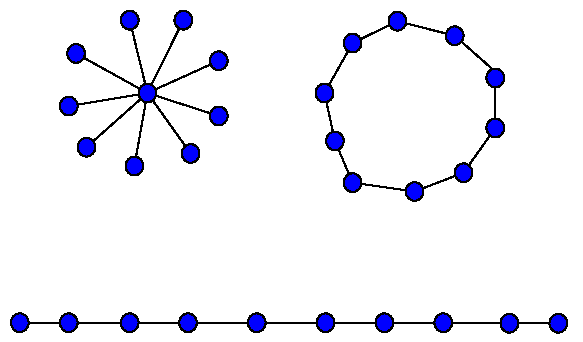
\includegraphics[width= \textwidth]{images/kernel-graphs.pdf}
		\caption{}
		\label{kernelgraphs}
	\end{subfigure}~
	\begin{subfigure}[b]{0.45\textwidth}
		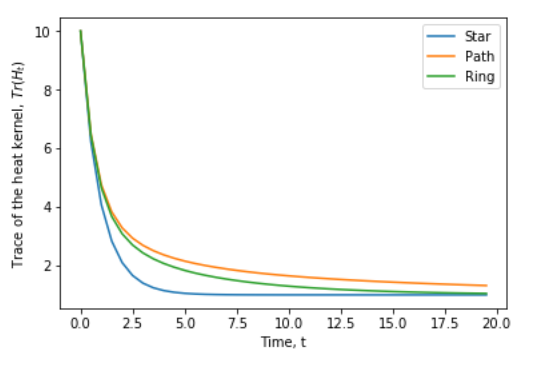
\includegraphics[width= \textwidth]{images/Trace-kernel-plot}
		\caption{}
		\label{plot-kernel}
	\end{subfigure}\\
	\begin{subfigure}[b]{0.45\textwidth}
		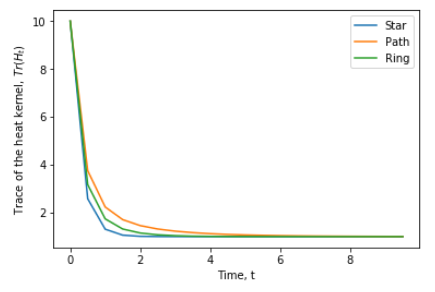
\includegraphics[width= \textwidth]{images/mellin-s-2.png}
		\caption{}
		\label{starpathmellins2}
	\end{subfigure}~
	\begin{subfigure}[b]{0.45\textwidth}
		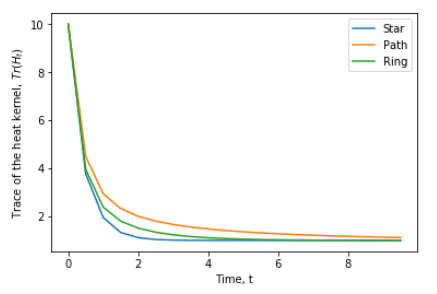
\includegraphics[width= \textwidth]{images/mellin-s-3.png}
		\caption{}
		\label{starpathmellins3}
	\end{subfigure}
	\caption{(\subref{kernelgraphs}) are the three graphs used for heat kernel analysis. (\subref{plot-kernel}) plot of the heat kernel trace against time for star (blue), path (orange) and regular(green) graphs. Figures (\subref{starpathmellins2}) and (\subref{starpathmellins3}) are the plots of trace function against time for the $3$ graphs based on the Mellin transforms of the $k$-Laplacians for $s=2$ and $s=3$ respectively.}
\end{figure}
From (\subref{plot-kernel}), we observe that since the $3$ graphs are different in terms of structure, the curves too take on different shapes. It is evident that since path and $2$-regular graphs have similar topologies, their corresponding graphs are close to each other while for star graph, its curve has a deeper trough. 
On comparing the plots for $s=2$ and $s=3$, we observe drastic shift in the curves for the former than the latter in comparison with the plot for the normal graph Laplacian in Fig.(\subref{plot-kernel}).

\section{The Generalised Laplacian Matrix}
In \cite{estrada2012path}, Estrada put forward the concept of the $k$-path Laplacian matrices which is based on the idea that one consider traversing a network by taking hops of length of $1, 2, \cdots, d_{max}$ where $d_{max}$ is the diameter of the network. The $k$-path Laplacian matrices are therefore a natural generalisation of the combinatorial Laplacian of a graph \cite{estrada2012path}. The motivation behind this generalisation is the idea of determining whether every node in a graph can be visited by means of a process that involves hopping from one node to another separated at a distance $k$. We can better understand the concept of $k$-path Laplacian by considering the analogy of polarisation process on a network as explained in \cite{estrada2012path}.  

Following \cite{estrada2017long}, we recall that the $k$-path Laplacian matrix $L_k(k \leq d_{max})$ of a connected undirected graph $G=(V,E)$ is defined as the square symmetric $n \times n$ matrix whose entries are given by:
\begin{eqnarray}
L_k(ij) = \begin{cases} -1 &\mbox{if } d_{i,j} = k, \\
\delta_k(i) &\mbox{if } i = j,  \\
0 & \text{otherwise},
\end{cases}
\end{eqnarray}\label{k-laplacian}
where $d_{i,j}$ is the shortest path distance between nodes $i$ and $j$, $\delta_{k}(i)$ known as the $k$-path degree is the number of irreducible shortest paths of length $k$ having node $i$ as an endpoint.\\

The $k$-path Laplacian matrices are real, symmetric, positive semi-definite matrices. In addition, $0$ is an eigenvalue of $\mathbf{L}_k$ with a $\mathbf{1}$ eigenvector that is, $\mathbf{L}_k \mathbf{1}^T = \mathbf{0}$ \cite{estrada2012path}.

For example, let us compute the $k$-path Laplacians for a simple graph $G$ in Fig.\ref{spanning}.

\begin{figure}[H]
	\centering
	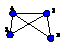
\includegraphics[width=0.25\textwidth]{images/compute-spanning.pdf}
	\caption{ A network of size 4.}
	\label{spanning}
\end{figure}


\begin{eqnarray*}
	\mathbf{L_1(G)} = \begin{pmatrix}
		2 & -1 & 0 & -1 \\
		-1 & 3 & -1 & -1 \\
		0 & -1 & 2 & -1  \\
		-1 & -1 & -1 & 3
	\end{pmatrix}, \quad
	\mathbf{L_2(G)} = \begin{pmatrix}
		1 & 0 & -1 & 0 \\
		0 & 0 & 0 & 0 \\
		-1 & 0 & 1 & 0 \\
		0 & 0 & 0 & 0
	\end{pmatrix}, \quad
	\mathbf{L_3(G)} = \begin{pmatrix}
		0 & 0 & 0 & 0 \\
		0 & 0 & 0 & 0 \\
		0 & 0 & 0 & 0 \\
		0 & 0 & 0 & 0
	\end{pmatrix}
\end{eqnarray*}


Using the $k$-path Laplacian, we can obtain an expression for the generalised Laplacian Matrix as a linear combination of the $k$-path Laplacian matrices given by 
\begin{equation}
L_{G} =  \Big(\sum_{k=1}^{d_{max}}c_k\mathbf{L}_{k} \Big) = c_{1}L_{1} + c_{2}L_{2} + \cdots + c_{d_{max}}L_{d_{max}}, 
\label{gen_lap}
\end{equation}
where $d_{max}$ is the diameter and $c_k$ are the co-efficients.

\section{Choice of co-efficients, $c_k$}
Considering the generalised Laplacian Matrix in Eqn.\ref{gen_lap}, the co-efficients $c_k$ are chosen in such a way that the effect of the long-range interactions weakens as the separation between nodes increases. The choice of the co-efficients $c_k$ is evident in many man-made and naturally evolving systems where communication among the agents of the system follows a spatial decay. For instance in sensor systems, sensors far away from the target display low noise-signal ratio as a result of attenuation (spatial decay) of signal energy, in earthquake incidences where the aftershocks follow a spatial decay, that is, areas further from the main shock are less affected compared to nearer areas. This spatial decay takes on the form $r ^{-\alpha}$ , where $r$ is the distance from the main shock. Other examples of similar physical scenarios include the brain in which the interconnectivity certain neurons in mammalian neo-cortex decays exponentially with the intersomatic distance, and many others.

In this paper, we consider two forms that the spatial decay can take on namely: 
\begin{enumerate}
	\item Exponential form
	
	For the exponential form, Eqn.\ref{gen_lap} attains a generalised form based on the Laplace-transformed $k$-Laplacian:
	\begin{equation}
	\tilde{\mathbf{L}}_{L,\lambda} = \mathbf{L} + \sum_{k=2}^{\Delta} e^{-\lambda k} \mathbf{L}_k, 
	\label{laplacetransform}
	\end{equation}
	where $\lambda >0$ is a parameter that depends on the specific situation to be modelled.
	Thus, the coefficients of Eqn.\ref{gen_lap} are $c_1 = 1$ and $c_{k \geq 2} = e^{-\lambda k}$.
	
	\item Power-law 
	
	Here, we use the Mellin transform of $k$-Laplacian matrices to obtain the generalised equation:
	\begin{equation}
	\tilde{\mathbf{L}}_{M,s} = \sum_{k=1}^{\Delta} k^{-s} \mathbf{L}_k,
	\label{mellin-transforms}
	\end{equation}
	where $s >0$ is a parameter that depends on the specific situation to be modelled and the coefficients of Eqn.\ref{gen_lap} are $c_{k} = k^{-s}$.     
\end{enumerate}

Following from the two transforms, we can then define the Laplacian matrix by
\begin{equation}
\mathbf{L}_{G} = \begin{cases} \sum_{d=1}^{d_{max}} k^{-s} L_d &\mbox{for } \tau = Mell, s>0 \\
L + \sum_{d=2}^{d_{max}} e^{-\lambda d} L_d   & \mbox{for } \tau = Lapl, \lambda>0. \end{cases} 
\end{equation}

\subsection{Properties of the Generalised Laplacian matrix, $L_G$}
\begin{prop}
	Real and Symmetric
	
	For $k=1,2,\cdots, d_{max}$, let $c_1 L_1,c_2 L_2, \cdots, c_{d_{max}} L_{d_{max}}$ be symmetric matrices of the same size. Consider $ L_G = c_1L_1+ c_2 L_2 + \cdots+ c_{d_{max}} c_{d_{max}} L_{d_{max}}$. Following the property of transposes; $ (c_1L_1+ c_2 L_2 + \cdots+ L_{d_{max}})^T =  c_1 L_1^T + c_2 L_2^T + \cdots+ c_{d_{max}} L_{d_{max}}^T$. Since $L_k$ are symmetric matrices, we know that for a given $k$, $L_{k} ^T = L_k$. Thus, $(c_1 L_1+ c_2 L_2 + \cdots+ c_{d_{max}} L_{d_{max}})^T = c_1 L_1+ c_2 L_2 + \cdots+ c_{d_{max}} L_{d_{max}}$ which implies $L_{G}^T = L_G$.
\end{prop}
\begin{prop}
	Positive-Semi definite
	\begin{proof}
		For any column vector $\mathbf{y}$
		\begin{equation}
		\mathbf{y}^T L_{G} \mathbf{y} = \mathbf{y}^T(c_{1}L_{1} + c_{2}L_{2} + \cdots + c_{\delta}L_{\delta} )\mathbf{y}
		= \mathbf{y}^Tc_{1}L_{1}\mathbf{y} + \mathbf{y}^Tc_{2}L_{2}\mathbf{y} + \cdots + \mathbf{y}^Tc_{\delta}L_{\delta}\mathbf{y} 
		\end{equation}
		Since $\mathbf{y}^Tc_{k}L_{k}\mathbf{y} \geq 0$ for $c_{k}>0$ and $1 \leq k \leq d_{max}$, then
		\begin{equation}
		\mathbf{y}^T L_{G} \mathbf{y} \geq 0	
		\end{equation}
	\end{proof}
\end{prop}
\begin{prop}
	Zero is an eigenvalue of $L_G$ with $1$ as an eigenvector.
	Let $\mathbf{v} = \mathbf{0}$, then $ L_G \mathbf{v} = (c_1L_1+ c_2 L_2 + \cdots+ c_{d_{max}} L_{d_{max}}) \mathbf{v}$ which gives
	\begin{equation}
	L_G \mathbf{v} = c_1 L_1 \mathbf{v} + c_2 L_2 \mathbf{v} + \cdots+ c_{d_{max}} L_{d_{max}} \mathbf{v}.
	\end{equation}
	since $c_k L_k \mathbf{v} =0$, Then $L_G \mathbf{v} = 0$ which implies that atleast $0$ is an eigenvalue of $L_G$ with $1$ as an eigenvector.
\end{prop}

\section{Generalised Heat Diffusion Model}
In the previous section, we have discussed the diffusion process that occurs through direct interactions between nearest neighbours in the network. In this section however, we consider the fact that in many real-world processes, it is observed that interactions with in networks do not only occur among nearest neighbours but also among non-nearest which we refer to as the long range interactions as illustrated in Fig.~\ref{long-range-demo}

\begin{figure}[H]
	\centering
	\begin{subfigure}[b]{0.3\textwidth}
		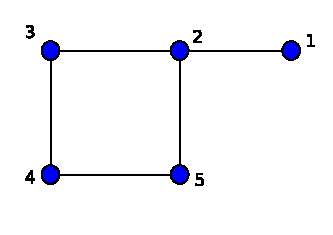
\includegraphics[width=\textwidth]{images/kenel-toymodel.pdf}
		\caption{}
		\label{toymodel}
	\end{subfigure}~
	\begin{subfigure}[b]{0.3\textwidth}
		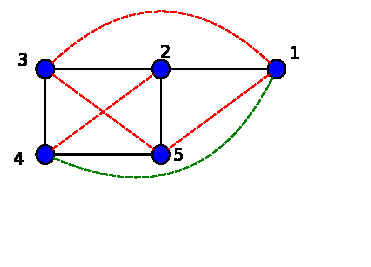
\includegraphics[width= \textwidth]{images/graph-longrange-demo.pdf}
		\caption{}
		\label{graph-longrange}
	\end{subfigure}
	\caption{(\subref{toymodel}) is a simple graph indicating the direct interactions followed in the normal diffusion model. (\subref{graph-longrange}) is a simple graph indicating both direct interactions (black solid lines), long-range interactions at hops of length $2$ (red broken lines) and $3$ (green-broken lines) that depict the generalised diffusion model.    }
	\label{long-range-demo}
\end{figure}


\subsection{The Generalised Heat Kernel}
The diffusion process accounting for the long-range interactions is defined by
%The heat equation in this case is based the the concept of $k$-path Laplacian introduced by Estrada \citep{estrada2012path} and is given by

\begin{equation}
\frac{d\boldsymbol{\phi}}{dt} =  -\varepsilon L_{G} \boldsymbol{\phi}, \quad \boldsymbol{\phi}(0) = \boldsymbol{\phi}_0 ,
\label{genheateq}
\end{equation}
where $L_G$ is the generalised Laplacian matrix.

The heat kernel $H_{Gt}$ of the generalised diffusion process which we refer to as the generalised heat kernel, the fundamental solution to eqn.\ref{genheateq} is given by 
\begin{equation}
H_{Gt} = e^{-L_{G}t},
\end{equation}
which on expansion can be written as 
\begin{equation}
H_{Gt} = e^{-t(c_{1}L_{1} + c_{2}L_{2} + \cdots + c_{\Delta}L_{\Delta})},
\end{equation}
where $L_1, L_2, \cdots, L{\Delta}$ are the matrices, known as $k$-path Laplacian matrices, which are obtained by considering hops of length $k=1,2,\cdots, \Delta$ respectively. At $k=1$, we recover the normal heat kernel in eqn.\ref{kernel}.

\subsection{Trace of the Generalised Heat Kernel}
The trace of the generalised heat kernel is therefore given by
\begin{equation}
Z_{G}(t) = Tr(H_{Gt}) = \sum_{i=1}^{|V|} e^{-\lambda_{iG} t}.
\label{Genkerneltrace}
\end{equation}
Alternatively, Eqn. \ref{Genkerneltrace} can be written as 
\begin{equation}
Z_{G}(t) =  1+ e^{-\lambda_{2G} t} + e^{-\lambda_{3G}} + \cdots + e^{-\lambda_{NG} t}
\end{equation}

\section{Experiments and Results}
Let us consider a simple graph in Fig.~\ref{toymodel}. We then perform simulation for normal diffusion as well as generalised diffusion on the graph. We compare results for generalised diffusion based on the Mellin and Laplace transforms for different values of $s$ and $\lambda$ respectively.
\begin{figure}[H]
	\centering
	\begin{subfigure}[b]{0.45\textwidth}
		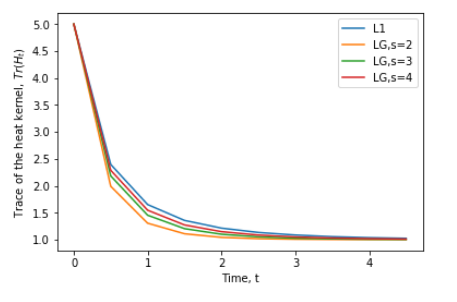
\includegraphics[width= \textwidth]{images/model-1-mellin.png}
		\caption{}
		\label{model1-mellin}
	\end{subfigure}~
	\begin{subfigure}[b]{0.45\textwidth}
		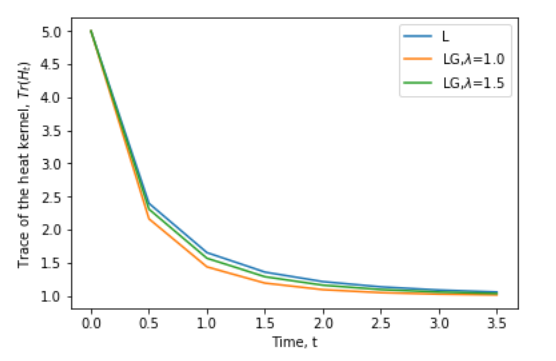
\includegraphics[width= \textwidth]{images/model-1-Laplace.png}
		\caption{}
		\label{model1-laplace}
	\end{subfigure} 
	\caption{(\subref{model1-mellin}) is a plot of the heat kernel function against time for mellin-transform diffusion on graph in Fig.~\ref{toymodel}. (\subref{model1-laplace}) is a plot of the heat kernel function against time for laplace -transform diffusion on graph in Fig.~\ref{toymodel}}
	\label{toy-mellin-laplace}
\end{figure}

From Fig.~\ref{toy-mellin-laplace}, we that for both cases, as the value of the parameters $s$ and $\lambda$ increases, the curve of the heat kernel function approaches that corresponding heat kernel function with no long-range interactions. 

\subsection{Comparison of Barabasi and E-R networks for Mellin and Laplace}
\newpage

\section{Zeta Function}

The Zeta function associated with the Laplacian eigenvalues is obtained by exponentiating and summing the reciprocal of the non-zero Laplacian eigenvalues. It is an invariant defined by
\begin{equation}
\zeta(s) = \sum_{\lambda_i \neq 0} \lambda_i ^{-s}.
\label{zeta-function}
\end{equation} 
In his work \cite{xiao2009graph}, Xiao established a relationship between the zeta function and the heat kernel trace by use of the Mellin transform. 
Applying the Mellin transform to the function $f(t)=e^{-\lambda_i t}$ gives 
\begin{equation}
\zeta(s) = \sum_{\lambda_i \neq 0} \lambda_i ^{-s} = \frac{1}{\Gamma(s)} \int_{0}^{\infty} t^{s-1} \sum_{\lambda_i \neq 0} e^{-\lambda_i t} dt = \frac{1}{\Gamma(s)} \int_{0}^{\infty} t^{s-1} \left \{ Tr(h_t)-C \right \} dt.
\label{label-kernel}
\end{equation}
where $\Gamma(s)$ is the gamma function defined as 
\begin{equation}
\Gamma(s) = \int_{0}^{\infty} t^{s-1} e^{-t} dt.
\end{equation}
where $C$ is the multiplicity of zero eigenvalues of the Laplacian that is the number of connected components of a graph.

Thus the zeta function is related to the moments of the heat kernel trace. It is the moment generating function and thus a way of characterising the shape of the heat kernel trace.

\subsection{Characterisation of shape of heat kernel Trace using the Zeta Function}

\subsection{Zeta Function Behaviour with exponent $s$}
In this subsection, we explore how the Zeta function varies with the exponent $s$. 
The zeta function Eqn.~\ref{zeta-function} can be written in as 
\begin{equation}
\zeta(s) = \frac{1}{\lambda_1^s}+ \frac{1}{\lambda_2^s}+ \frac{1}{\lambda_3^s} + \cdots + \frac{1}{\lambda_n^s} 
\end{equation} 
for $\lambda_i > 0$.
Two cases arise as $s$ values changes that is for $\lambda_i < 1$, as $s$ increases,  the value $\frac{1}{\lambda_i^s}$ increases. However on the otherhand, for $\lambda_i > 1$, as $s$ increases,  the value $\frac{1}{\lambda_i^s}$ decreases. In otherwords, as $s$ gets large, the behaviour of the zeta function is completely determined the eigenvalues with small values. This is evident in the simulations of the zeta function as follows:
\begin{figure}[H]
	\centering
	\begin{subfigure}[b]{0.35\textwidth}
		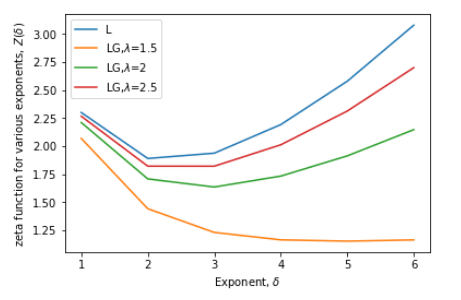
\includegraphics[width= \textwidth]{images/zeta-laplace.png}
		\caption{}
		\label{zeta-laplace}
	\end{subfigure}~
	\begin{subfigure}[b]{0.35\textwidth}
		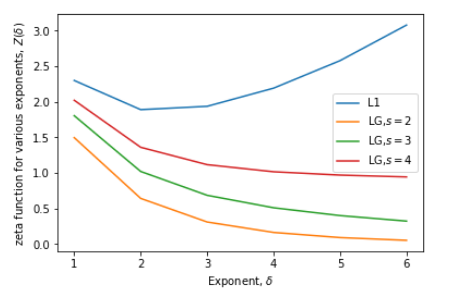
\includegraphics[width= \textwidth]{images/zeta-mellin.png}
		\caption{}
		\label{zeta-mellin}
	\end{subfigure} 
	\caption{Illustration of the Zeta function of the graph in Fig.~\ref{keneltoymodel1} against exponent $\delta$. (\subref{zeta-laplace}) corresponds to the Laplace transform of the graph Laplacian with $\lambda = 1.5, 2,$ and $2.5$. (\subref{zeta-mellin}) corresponds to the Mellin transform of the graph Laplacian with $s = 2, 3,$ and $4$. }
	\label{}
\end{figure}

Looking at the curves in Fig.~\ref{zeta-laplace}, we observe that the curves corresponding to the Laplacian transforms approach the curve of the normal Laplacian as $\lambda$ becomes increases. In addition, we observe that the curves for $\lambda=2$ and $2.5$ take on a similar shape as that of the 'classical' Laplacian while the curve for $\lambda=1.5$ takes on a different shape as the $s$ becomes large. this can be explained following from the fact as $s$ becomes large, the behaviour of the zeta function is determined by the small non-zero eigenvalues of the Laplacian. Let us consider

\subsection{Derivative of Zeta Function at the Origin}

The derivative or slope of the zeta function at the origin is another characterisation of the heat kernel trace second to the zeta function which measures it's shape.

Thus, the derivative is given by
\begin{equation}
\zeta'(s) = \sum_{\lambda_i \neq 0} \{-\ln \lambda_i\}
e^{-s \ln \lambda_i}
\end{equation}
so, the derivative at the origin is 
\begin{equation}
\zeta'(s) = -\sum_{\lambda_i \neq 0}\ln \lambda_i
\end{equation}

\section{Heat Content}

The heat content is defined as the sum of the entries of the heat kernel matrix of a graph. Its given by
\begin{equation}
Q(t) = \sum_{u \in V} \sum_{v \in V} h_{t}(u,v)
\end{equation}
Substituting for $h_t(u,v)$ gives
\begin{equation}
Q(t) = \sum_{p \in V} \sum_{q \in V} \sum_{k=1}^{\arrowvert V\arrowvert} e^{(-\lambda_{k} t)} v_{k}(p) v_{k}(q),
\end{equation}
which can be expanded into a polynomial in time as in \cite{mcdonald2002diffusions}
\begin{equation}
Q(t) = \sum_{m=0}^{\infty} q_m t^m
\end{equation}

\begin{Th} \label{main} Every beginning is hard. But once you are familiar with latex, you won't use Microsoft Words again for creating mathematical papers.
\end{Th}

\section{Proof of Theorem~\ref{main}}

In this section we present the proof of Theorem~\ref{main}.

\begin{proof} We leave the proof of the first statement to the Reader. Now we prove the second statement. The main advantage of latex is that it is much easier to create mathematical formulas and they look much better than in Microsoft Word.
For instance,
$$\frac{x^2+1}{\sqrt{u+v}}\in \mathbb{R}.$$
On the other, you can do everything which can be done with Microsoft Word. You can put pictures in it, but generally you can only indicate its place, the actual place of the figure depends on many things. For instance, in the latex file there is a picture following this sentence, but since there is no place here, the program will take it to the next page, and some texts precede it. If you have problem with some figure, don't hesitate to ask me.

%\begin{figure}[h!]
%\scalebox{.45}{\includegraphics{hexagonal_lattice.eps}}  
%\end{figure}

From time to time, you will need some commands. Practically, I use at most 20 commands regularly, and sometimes I need tricky command which I find on the internet. I emphasize again that if you have any question, feel free to ask me.

\end{proof}

\begin{thebibliography}{99} 

\bibitem{newman2010} Newman, M., 2010. Networks: an introduction. Oxford university press.

\bibitem{estrada2011epidemic} Estrada, E., Kalala-Mutombo, F. and Valverde-Colmeiro, A., 2011. Epidemic spreading in networks with nonrandom long-range interactions. Physical Review E, 84(3), p.036110.

\bibitem{kasprzak2012diffusion} Kasprzak, R., 2012. Diffusion in networks. Journal of Telecommunications and Information Technology, pp.99-106.

\bibitem{lopez2008diffusion} L�pez-Pintado, D., 2008. Diffusion in complex social networks. Games and Economic Behavior, 62(2), pp.573-590.

\bibitem{estrada2012path} Estrada, E., 2012. Path Laplacian matrices: introduction and application to the analysis of consensus in networks. Linear Algebra and its Applications, 436(9), pp.3373-3391.

\bibitem{estrada2017long} Estrada, E., Hameed, E., Hatano, N. and Langer, M., 2017. Path Laplacian operators and superdiffusive processes on graphs. I. One-dimensional case. Linear Algebra and its Applications, 523, pp.307-334.

\bibitem{xiao2007kernel}Bai, X., 2007. Heat Kernal Analysis on Graphs. University of York, Department of Computer Science.

\bibitem{xiao2009graph} Xiao, B., Hancock, E.R. and Wilson, R.C., 2009. Graph characteristics from the heat kernel trace. Pattern Recognition, 42(11), pp.2589-2606.


\bibitem{edwards2004differential} Edwards, C.H., Penney, D.E. and Calvis, D.T., 2004. Differential equations and boundary value problems. 

\bibitem{estrada2017sync} Estrada, E., Gambuzza, L.V. and Frasca, M., 2018. Long-Range Interactions and Network Synchronization. SIAM Journal on Applied Dynamical Systems, 17(1), pp.672-693.

\bibitem{mcdonald2002diffusions} McDonald, P. and Meyers, R., 2002. Diffusions on graphs, Poisson problems and spectral geometry. Transactions of the American Mathematical Society, 354(12), pp.5111-5136.

\bibitem{wiki} \begin{verbatim} http://en.wikibooks.org/wiki/LaTeX \end{verbatim}



\end{thebibliography}



\end{document}